\documentclass[10pt]{article}
\usepackage[polish]{babel}
\usepackage[utf8]{inputenc}
\usepackage[T1]{fontenc}
\usepackage{graphicx}
\usepackage[export]{adjustbox}
\graphicspath{ {./images/} }
\usepackage{amsmath}
\usepackage{amsfonts}
\usepackage{amssymb}
\usepackage[version=4]{mhchem}
\usepackage{stmaryrd}
\usepackage{hyperref}
\hypersetup{colorlinks=true, linkcolor=blue, filecolor=magenta, urlcolor=cyan,}
\urlstyle{same}
\usepackage{multirow}

\title{KOD PESEL }

\author{}
\date{}


\begin{document}
\maketitle
\begin{center}
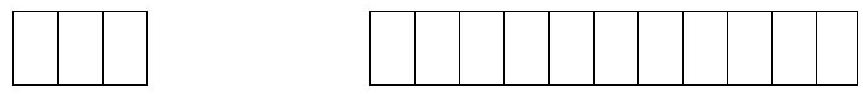
\includegraphics[max width=\textwidth]{2024_11_21_94f02db55673a8a7b820g-01}
\end{center}

\section*{PRÓBNY EGZAMIN MATURALNY}
Marzec 2017

\section*{Z MATEMATYKI \\
 POZIOM PODSTAWOWY}
\begin{enumerate}
  \item Sprawdź, czy arkusz egzaminacyjny zawiera 20 stron (zadania 1-33). Ewentualny brak zgłoś przewodniczącemu zespołu nadzorującego próbny egzamin.
  \item Rozwiązania zadań i odpowiedzi wpisuj w miejscu na to przeznaczonym.
  \item Odpowiedzi do zadań zamkniętych (1-23) zaznacz kółkiem. Błędne zaznaczenie przekreśl i zaznacz właściwe.
  \item Pamiętaj, że pominięcie argumentacji lub istotnych obliczeń w rozwiązaniu zadania otwartego (24-33) może spowodować, że za to rozwiązanie nie będziesz mógł dostać pełnej liczby punktów.
  \item Pisz czytelnie i używaj tylko długopisu lub pióra z czarnym tuszem lub atramentem.
  \item Nie używaj korektora, a błędne zapisy wyraźnie przekreśl.
  \item Pamiętaj, że zapisy w brudnopisie nie będą oceniane.
  \item Możesz korzystać z zestawu wzorów matematycznych, cyrkla i linijki oraz kalkulatora.
  \item Na karcie odpowiedzi wpisz swój numer PESEL.
\end{enumerate}

\section*{ZADANIA ZAMKNIETE}
\section*{W zadaniach od 1. do 23. wybierz i przenieś na kartę poprawnq odpowiedź.}
\section*{Zadanie 1.}
Pewien towar kosztował \(600 \mathrm{zł}\). Jego cenę obniżono o \(15 \%\), a następnie w ramach wyprzedaży sezonowej obniżono o kolejne 10\%. Po obu obniżkach towar kosztuje:\\
A. \(450 \mathrm{zł}\)\\
B. \(459 \mathrm{zł}\)\\
C. \(561 \mathrm{zł}\)\\
D. \(621 \mathrm{zł}\)

Zadanie 2.\\
Liczba \(\left(\frac{3+\sqrt{3}}{\sqrt{3}}\right)^{2}\) jest równa:\\
A. 4\\
B. 9\\
C. \(\frac{3+\sqrt{3}}{3}\)\\
D. \(4+2 \sqrt{3}\)

\section*{Zadanie 3.}
Zbiorem wartości funkcji, której wykres jest przedstawiony na rysunku jest przedział:\\
A. \(\langle-4,5\rangle\)\\
B. \(\langle-4,5)\)\\
C. \(\langle-2,3\rangle\)\\
D. \(\langle-2,3)\)\\
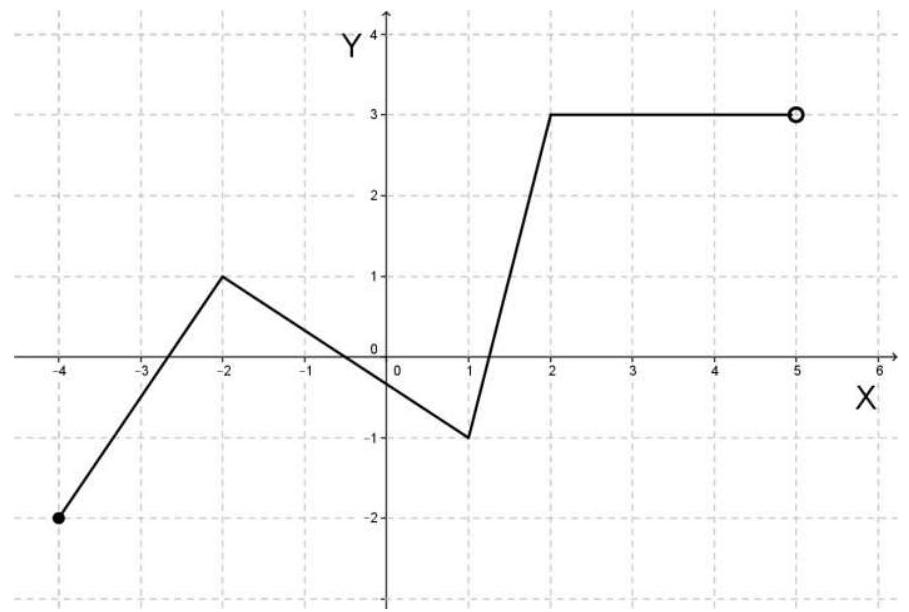
\includegraphics[max width=\textwidth, center]{2024_11_21_94f02db55673a8a7b820g-02}

\section*{Zadanie 4.}
Liczba dodatnich wyrazów ciągu o wyrazie ogólnym \(a_{n}=-2(n+1)(n-4)\) jest równa:\\
A. 3\\
B. 4\\
C. 5\\
D. 6

\section*{Zadanie 5.}
Do prostej należy początek układu współzzędnych oraz punkt \(P=(-8 ; 15)\). Wówczas cosinus kąta nachylenia tej prostej do osi \(O X\) jest równy:\\
A. \(-\frac{15}{17}\)\\
B. \(-\frac{8}{17}\)\\
C. \(\frac{8}{17}\)\\
D. \(\frac{15}{17}\)

\section*{BRUDNOPIS}
\begin{center}
\begin{tabular}{|c|c|c|c|c|c|c|c|c|c|c|c|c|c|c|c|c|c|c|c|c|c|c|c|}
\hline
 &  &  &  &  &  &  &  &  &  &  &  &  &  &  &  &  &  &  &  &  &  &  &  \\
\hline
 &  &  &  &  &  &  &  &  &  &  &  &  &  &  &  &  &  &  &  &  &  &  &  \\
\hline
 &  &  &  &  &  &  &  &  &  &  &  &  &  &  &  &  &  &  &  &  &  &  &  \\
\hline
 &  &  &  &  &  &  &  &  &  &  &  &  &  &  &  &  &  &  &  &  &  &  &  \\
\hline
 &  &  &  &  &  &  &  &  &  &  &  &  &  &  &  &  &  &  &  &  &  &  &  \\
\hline
 &  &  &  &  &  &  &  &  &  &  &  &  &  &  &  &  &  &  &  &  &  &  &  \\
\hline
 &  &  &  &  &  &  &  &  &  &  &  &  &  &  &  &  &  &  &  &  &  &  &  \\
\hline
 &  &  &  &  &  &  &  &  &  &  &  &  &  &  &  &  &  &  &  &  &  &  &  \\
\hline
 &  &  &  &  &  &  &  &  &  &  &  &  &  &  &  &  &  &  &  &  &  &  &  \\
\hline
 &  &  &  &  &  &  &  &  &  &  &  &  &  &  &  &  &  &  &  &  &  &  &  \\
\hline
 &  &  &  &  &  &  &  &  &  &  &  &  &  &  &  &  &  &  &  &  &  &  &  \\
\hline
 &  &  &  &  &  &  &  &  &  &  &  &  &  &  &  &  &  &  &  &  &  &  &  \\
\hline
 &  &  &  &  &  &  &  &  &  &  &  &  &  &  &  &  &  &  &  &  &  &  &  \\
\hline
 &  &  &  &  &  &  &  &  &  &  &  &  &  &  &  &  &  &  &  &  &  &  &  \\
\hline
 &  &  &  &  &  &  &  &  &  &  &  &  &  &  &  &  &  &  &  &  &  &  &  \\
\hline
 &  &  &  &  &  &  &  &  &  &  &  &  &  &  &  &  &  &  &  &  &  &  &  \\
\hline
 &  &  &  &  &  &  &  &  &  &  &  &  &  &  &  &  &  &  &  &  &  &  &  \\
\hline
 &  &  &  &  &  &  &  &  &  &  &  &  &  &  &  &  &  &  &  &  &  &  &  \\
\hline
 &  &  &  &  &  &  &  &  &  &  &  &  &  &  &  &  &  &  &  &  &  &  &  \\
\hline
 &  &  &  &  &  &  &  &  &  &  &  &  &  &  &  &  &  &  &  &  &  &  &  \\
\hline
 &  &  &  &  &  &  &  &  &  &  &  &  &  &  &  &  &  &  &  &  &  &  &  \\
\hline
 &  &  &  &  &  &  &  &  &  &  &  &  &  &  &  &  &  &  &  &  &  &  &  \\
\hline
 &  &  &  &  &  &  &  &  &  &  &  &  &  &  &  &  &  &  &  &  &  &  &  \\
\hline
 &  &  &  &  &  &  &  &  &  &  &  &  &  &  &  &  &  &  &  &  &  &  &  \\
\hline
 &  &  &  &  &  &  &  &  &  &  &  &  &  &  &  &  &  &  &  &  &  &  &  \\
\hline
 &  &  &  &  &  &  &  &  &  &  &  &  &  &  &  &  &  &  &  &  &  &  &  \\
\hline
 &  &  &  &  &  &  &  &  &  &  &  &  &  &  &  &  &  &  &  &  &  &  &  \\
\hline
 &  &  &  &  &  &  &  &  &  &  &  &  &  &  &  &  &  &  &  &  &  &  &  \\
\hline
 &  &  &  &  &  &  &  &  &  &  &  &  &  &  &  &  &  &  &  &  &  &  &  \\
\hline
 &  &  &  &  &  &  &  &  &  &  &  &  &  &  &  &  &  &  &  &  &  &  &  \\
\hline
 &  &  &  &  &  &  &  &  &  &  &  &  &  &  &  &  &  &  &  &  &  &  &  \\
\hline
 &  &  &  &  &  &  &  &  &  &  &  &  &  &  &  &  &  &  &  &  &  &  &  \\
\hline
 &  &  &  &  &  &  &  &  &  &  &  &  &  &  &  &  &  &  &  &  &  &  &  \\
\hline
 &  &  &  &  &  &  &  &  &  &  &  &  &  &  &  &  &  &  &  &  &  &  &  \\
\hline
 &  &  &  &  &  &  &  &  &  &  &  &  &  &  &  &  &  &  &  &  &  &  &  \\
\hline
 &  &  &  &  &  &  &  &  &  &  &  &  &  &  &  &  &  &  &  &  &  &  &  \\
\hline
 &  &  &  &  &  &  &  &  &  &  &  &  &  &  &  &  &  &  &  &  &  &  &  \\
\hline
 &  &  &  &  &  &  &  &  &  &  &  &  &  &  &  &  &  &  &  &  &  &  &  \\
\hline
 &  &  &  &  &  &  &  &  &  &  &  &  &  &  &  &  &  &  &  &  &  &  &  \\
\hline
 &  &  &  &  &  &  &  &  &  &  &  &  &  &  &  &  &  &  &  &  &  &  &  \\
\hline
 &  &  &  &  &  &  &  &  &  &  &  &  &  &  &  &  &  &  &  &  &  &  &  \\
\hline
 &  &  &  &  &  &  &  &  &  &  &  &  &  &  &  &  &  &  &  &  &  &  &  \\
\hline
 &  &  &  &  &  &  &  &  &  &  &  &  &  &  &  &  &  &  &  &  &  &  &  \\
\hline
 &  &  &  &  &  &  &  &  &  &  &  &  &  &  &  &  &  &  &  &  &  &  &  \\
\hline
\end{tabular}
\end{center}

\section*{Zadanie 6.}
Poniżej przestawiony jest fragment wykresu funkcji kwadratowej. Funkcja ta ma wzór:\\
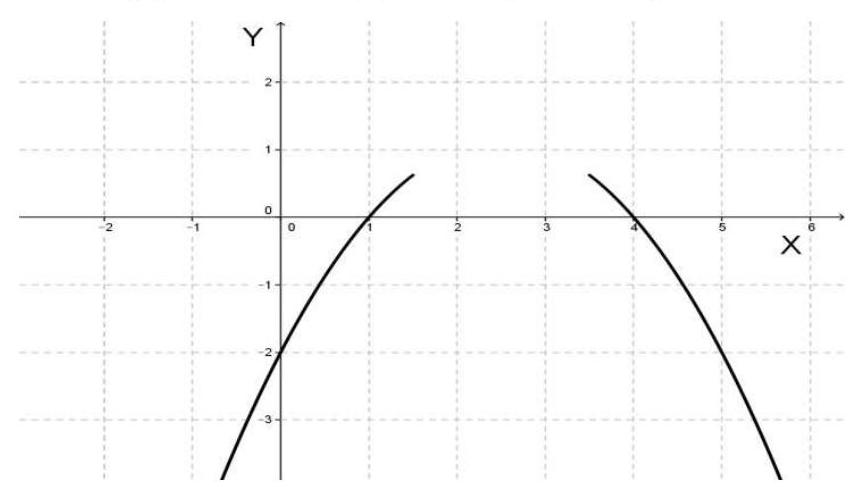
\includegraphics[max width=\textwidth, center]{2024_11_21_94f02db55673a8a7b820g-04}\\
A. \(f(x)=-\frac{1}{2} x^{2}+\frac{5}{2} x+2\)\\
B. \(\quad f(x)=-\frac{1}{2} x^{2}+\frac{5}{2} x-2\)\\
C. \(f(x)=-\frac{1}{2} x^{2}-\frac{5}{2} x+2\)\\
D. \(\quad f(x)=-\frac{1}{2} x^{2}-\frac{5}{2} x-2\)

\section*{Zadanie 7.}
Liczba \(32^{\frac{2}{5}} \cdot 16^{-\frac{3}{4}} \cdot\left(0,125^{\frac{1}{12}}\right)^{-4}\) jest równa:\\
A. 1\\
B. 4\\
C. 64\\
D. 80

\section*{Zadanie 8.}
Dana jest prosta \(m\) o równaniu \(y=-\frac{1}{3} x-2\). Prosta \(k\) równoległa do prostej \(m\) i przechodząca przez punkt \(P\) o współrzędnych \(P=(-3,-5)\) ma równanie:\\
A. \(y=3 x+4\)\\
B. \(y=-\frac{1}{3} x-6\)\\
C. \(y=\frac{1}{3} x-4\)\\
D. \(y=-3 x-14\)

\section*{Zadanie 9.}
Janek w pierwszym semestrze otrzymał następujące oceny z matematyki: z prac klasowych 2,3,3,4, z kartkówek 5,5,4,4,5,5, z odpowiedzi ustnych 2,3,4. Oceny z prac klasowych mają wagę 0,5 , z kartkówek 0,3 , z odpowiedzi ustnych 0,2 . Średnia ważona (zaokrąglona do dwóch miejsc po przecinku) ocen z matematyki Janka w pierwszym semestrze jest równa:\\
A. 3,68\\
B. 3,58\\
C. 3,25\\
D. 1,23

\section*{BRUDNOPIS}
Materiały pobrane z serwisu \href{http://www.zadania.info}{www.zadania.info}\\

\includegraphics[max width=\textwidth, center]{2024_11_21_94f02db55673a8a7b820g-05}

\section*{Zadanie 10.}
Dany jest kąt \(A B D\) o mierze \(29^{\circ}\) (rys.). Kąt \(B C D\) ma miarę:\\
A. \(29^{\circ}\)\\
B. \(69^{\circ}\)\\
C. \(61^{\circ}\)\\
D. \(58^{\circ}\)\\
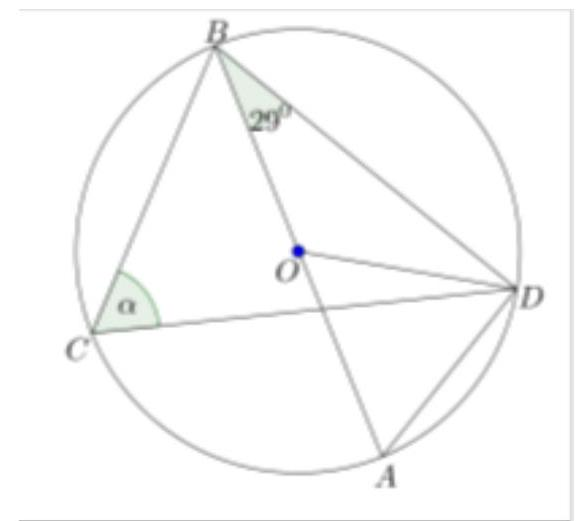
\includegraphics[max width=\textwidth, center]{2024_11_21_94f02db55673a8a7b820g-06}

\section*{Zadanie 11.}
Odległość punktu \(A=(3,-4)\) od jego obrazu w symetrii względem początku układu współrzędnych jest równa:\\
A. 6\\
B. 7\\
C. 8\\
D. 10

\section*{Zadanie 12.}
Wartość wyrażenia \(\frac{4 \log _{2} 2 \sqrt{2}+\log _{2} \frac{1}{8}}{\log _{3} 45-\log _{3} 5}\) jest równa:\\
A. \(\frac{3}{2}\)\\
B. 1\\
C. \(\frac{8}{9}\)\\
D. \(\frac{9}{2}\)

\section*{Zadanie 13.}
Suma \(n\) początkowych wyrazów ciągu \(\left(a_{n}\right)\) jest wyrażona wzorem \(S_{n}=n^{2}+3 n\). Drugi wyraz tego ciągu jest równy:\\
A. 16\\
B. \(\frac{3}{2}\)\\
C. 6\\
D. -9

\section*{Zadanie 14.}
Symetralna odcinka \(A B\), gdzie \(A=(-2,4), B=(3,-6)\) ma równanie:\\
A. \(y=\frac{1}{2} x+\frac{3}{4}\)\\
B. \(y=-\frac{1}{2} x-\frac{3}{4}\)\\
C. \(y=\frac{1}{2} x-\frac{5}{4}\)\\
D. \(y=2 x-2\)

\section*{Zadanie 15.}
Zbiorem wszystkich rozwiązań równania \(-2 x(3 x+1)(2-3 x)=0\) jest:\\
A. \(\left\{-\frac{1}{3} ; \frac{2}{3}\right\}\)\\
B. \(\left\{-\frac{1}{3} ; 0 ; \frac{2}{3}\right\}\)\\
C. \(\left\{-2 ;-\frac{1}{3} ; \frac{2}{3}\right\}\)\\
D. \(\left\{-2 ;-\frac{1}{3} ; 0 ; \frac{2}{3}\right\}\)\\

\includegraphics[max width=\textwidth, center]{2024_11_21_94f02db55673a8a7b820g-07}

\section*{Zadanie 16.}
Kąt nachylenia przekątnej ściany bocznej graniastosłupa prawidłowego trójkątnego do sąsiedniej ściany bocznej przedstawiono na rysunku:\\
A.\\
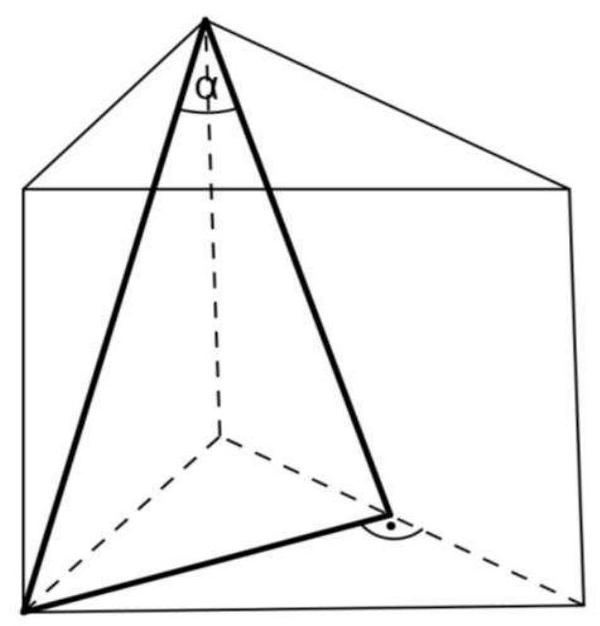
\includegraphics[max width=\textwidth, center]{2024_11_21_94f02db55673a8a7b820g-08(1)}\\
C.\\
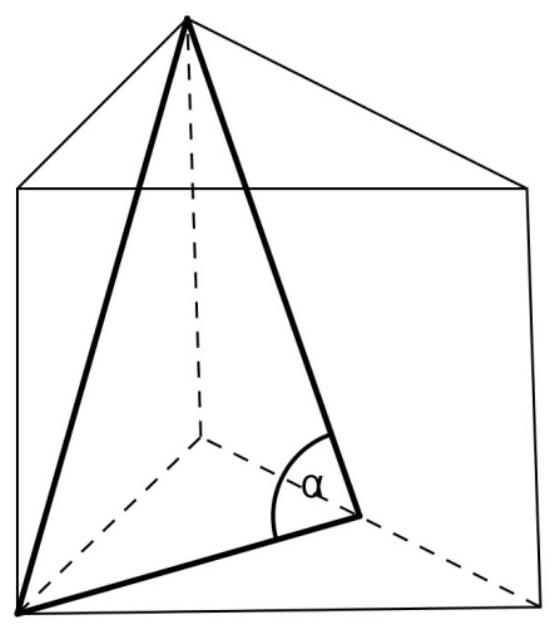
\includegraphics[max width=\textwidth, center]{2024_11_21_94f02db55673a8a7b820g-08(2)}\\
B.\\
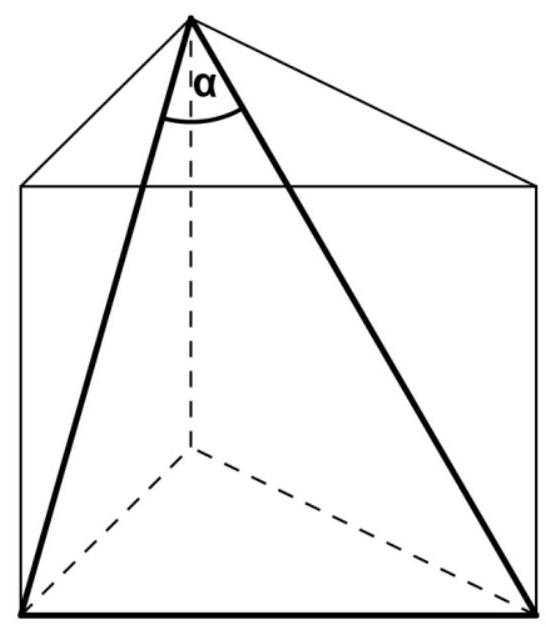
\includegraphics[max width=\textwidth, center]{2024_11_21_94f02db55673a8a7b820g-08(3)}\\
D.\\
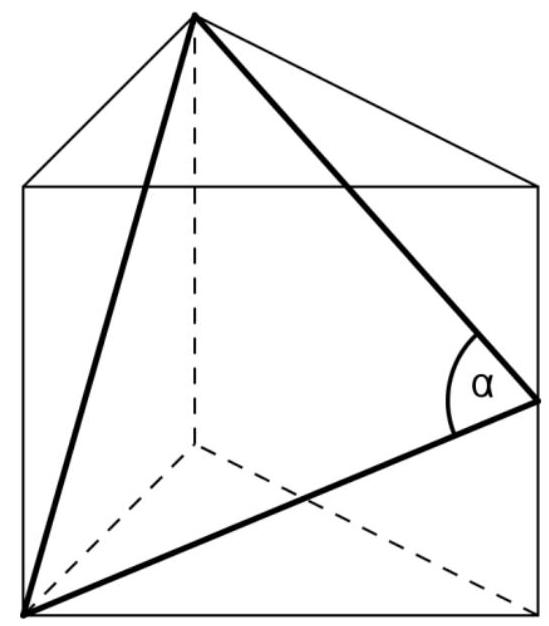
\includegraphics[max width=\textwidth, center]{2024_11_21_94f02db55673a8a7b820g-08}

\section*{Zadanie 17.}
Do wykresu funkcji liniowej należą punkty \(A=(-1,-5), B=(-3,7)\), zatem funkcja liniowa ma wzór:\\
A. \(f(x)=-\frac{1}{6} x-5\)\\
B. \(f(x)=-\frac{1}{2} x-5 \frac{1}{2}\)\\
C. \(f(x)=-6 x-11\)\\
D. \(f(x)=-2 x+7\)

\section*{BRUDNOPIS}
\begin{center}
\begin{tabular}{|c|c|c|c|c|c|c|c|c|c|c|c|c|c|c|c|c|c|c|c|c|c|c|c|}
\hline
 &  &  &  &  &  &  &  &  &  &  &  &  &  &  &  &  &  &  &  &  &  &  &  \\
\hline
 &  &  &  &  &  &  &  &  &  &  &  &  &  &  &  &  &  &  &  &  &  &  &  \\
\hline
 &  &  &  &  &  &  &  &  &  &  &  &  &  &  &  &  &  &  &  &  &  &  &  \\
\hline
 &  &  &  &  &  &  &  &  &  &  &  &  &  &  &  &  &  &  &  &  &  &  &  \\
\hline
 &  &  &  &  &  &  &  &  &  &  &  &  &  &  &  &  &  &  &  &  &  &  &  \\
\hline
 &  &  &  &  &  &  &  &  &  &  &  &  &  &  &  &  &  &  &  &  &  &  &  \\
\hline
 &  &  &  &  &  &  &  &  &  &  &  &  &  &  &  &  &  &  &  &  &  &  &  \\
\hline
 &  &  &  &  &  &  &  &  &  &  &  &  &  &  &  &  &  &  &  &  &  &  &  \\
\hline
 &  &  &  &  &  &  &  &  &  &  &  &  &  &  &  &  &  &  &  &  &  &  &  \\
\hline
 &  &  &  &  &  &  &  &  &  &  &  &  &  &  &  &  &  &  &  &  &  &  &  \\
\hline
 &  &  &  &  &  &  &  &  &  &  &  &  &  &  &  &  &  &  &  &  &  &  &  \\
\hline
 &  &  &  &  &  &  &  &  &  &  &  &  &  &  &  &  &  &  &  &  &  &  &  \\
\hline
 &  &  &  &  &  &  &  &  &  &  &  &  &  &  &  &  &  &  &  &  &  &  &  \\
\hline
 &  &  &  &  &  &  &  &  &  &  &  &  &  &  &  &  &  &  &  &  &  &  &  \\
\hline
 &  &  &  &  &  &  &  &  &  &  &  &  &  &  &  &  &  &  &  &  &  &  &  \\
\hline
 &  &  &  &  &  &  &  &  &  &  &  &  &  &  &  &  &  &  &  &  &  &  &  \\
\hline
 &  &  &  &  &  &  &  &  &  &  &  &  &  &  &  &  &  &  &  &  &  &  &  \\
\hline
 &  &  &  &  &  &  &  &  &  &  &  &  &  &  &  &  &  &  &  &  &  &  &  \\
\hline
 &  &  &  &  &  &  &  &  &  &  &  &  &  &  &  &  &  &  &  &  &  &  &  \\
\hline
 &  &  &  &  &  &  &  &  &  &  &  &  &  &  &  &  &  &  &  &  &  &  &  \\
\hline
 &  &  &  &  &  &  &  &  &  &  &  &  &  &  &  &  &  &  &  &  &  &  &  \\
\hline
 &  &  &  &  &  &  &  &  &  &  &  &  &  &  &  &  &  &  &  &  &  &  &  \\
\hline
 &  &  &  &  &  &  &  &  &  &  &  &  &  &  &  &  &  &  &  &  &  &  &  \\
\hline
 &  &  &  &  &  &  &  &  &  &  &  &  &  &  &  &  &  &  &  &  &  &  &  \\
\hline
 &  &  &  &  &  &  &  &  &  &  &  &  &  &  &  &  &  &  &  &  &  &  &  \\
\hline
 &  &  &  &  &  &  &  &  &  &  &  &  &  &  &  &  &  &  &  &  &  &  &  \\
\hline
 &  &  &  &  &  &  &  &  &  &  &  &  &  &  &  &  &  &  &  &  &  &  &  \\
\hline
 &  &  &  &  &  &  &  &  &  &  &  &  &  &  &  &  &  &  &  &  &  &  &  \\
\hline
 &  &  &  &  &  &  &  &  &  &  &  &  &  &  &  &  &  &  &  &  &  &  &  \\
\hline
 &  &  &  &  &  &  &  &  &  &  &  &  &  &  &  &  &  &  &  &  &  &  &  \\
\hline
 &  &  &  &  &  &  &  &  &  &  &  &  &  &  &  &  &  &  &  &  &  &  &  \\
\hline
 &  &  &  &  &  &  &  &  &  &  &  &  &  &  &  &  &  &  &  &  &  &  &  \\
\hline
 &  &  &  &  &  &  &  &  &  &  &  &  &  &  &  &  &  &  &  &  &  &  &  \\
\hline
 &  &  &  &  &  &  &  &  &  &  &  &  &  &  &  &  &  &  &  &  &  &  &  \\
\hline
 &  &  &  &  &  &  &  &  &  &  &  &  &  &  &  &  &  &  &  &  &  &  &  \\
\hline
 &  &  &  &  &  &  &  &  &  &  &  &  &  &  &  &  &  &  &  &  &  &  &  \\
\hline
 &  &  &  &  &  &  &  &  &  &  &  &  &  &  &  &  &  &  &  &  &  &  &  \\
\hline
 &  &  &  &  &  &  &  &  &  &  &  &  &  &  &  &  &  &  &  &  &  &  &  \\
\hline
 &  &  &  &  &  &  &  &  &  &  &  &  &  &  &  &  &  &  &  &  &  &  &  \\
\hline
 &  &  &  &  &  &  &  &  &  &  &  &  &  &  &  &  &  &  &  &  &  &  &  \\
\hline
 &  &  &  &  &  &  &  &  &  &  &  &  &  &  &  &  &  &  &  &  &  &  &  \\
\hline
 &  &  &  &  &  &  &  &  &  &  &  &  &  &  &  &  &  &  &  &  &  &  &  \\
\hline
 &  &  &  &  &  &  &  &  &  &  &  &  &  &  &  &  &  &  &  &  &  &  &  \\
\hline
 &  &  &  &  &  &  &  &  &  &  &  &  &  &  &  &  &  &  &  &  &  &  &  \\
\hline
\end{tabular}
\end{center}

\section*{Zadanie 18.}
Którym wzorem ogólnym przedstawiono ciąg geometryczny?\\
A. \(a_{n}=\left(\frac{1}{3}\right)^{n}+\left(\frac{1}{2}\right)^{n}\)\\
B. \(a_{n}=\frac{2 n-4}{4}\)\\
C. \(a_{n}=5 n^{2}\)\\
D. \(a_{n}=\frac{3^{n}}{5^{n+1}}\)

Zadanie 19.\\
Wartość wyrażenia \(\sqrt{\frac{4 \cos { }^{2} 30^{\circ}+\operatorname{tg} 30^{\circ} \cdot \operatorname{tg} 60^{\circ}}{\sin ^{2} 33^{\circ}+\sin ^{2} 57^{\circ}}}+\operatorname{tg} 45^{\circ}\) jest równa:\\
A. 2\\
B. \(\sqrt{2}\)\\
C. 3\\
D. \(\frac{2}{\sin 33^{\circ}+\sin 57^{\circ}}+1\)

\section*{Zadanie 20.}
Wszystkich liczb naturalnych pięciocyfrowych, w których cyfrą jedności jest 4, cyfra setek jest liczba nieparzystą, a cyfra tysięcy jest liczbą podzielną przez 3 jest:\\
A. \(9 \cdot 4 \cdot 5 \cdot 9 \cdot 4\)\\
B. \(9 \cdot 4 \cdot 5 \cdot 10 \cdot 1\)\\
C. \(10 \cdot 4 \cdot 5 \cdot 10 \cdot 1\)\\
D. \(9 \cdot 3 \cdot 5 \cdot 10 \cdot 1\)

\section*{Zadanie 21.}
Na rysunkach przedstawione są wykresy funkcji \(f\) i \(g\).\\
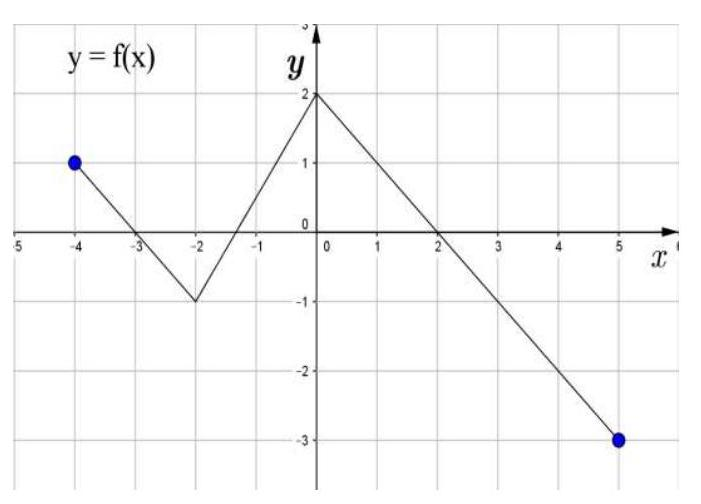
\includegraphics[max width=\textwidth, center]{2024_11_21_94f02db55673a8a7b820g-10}\\
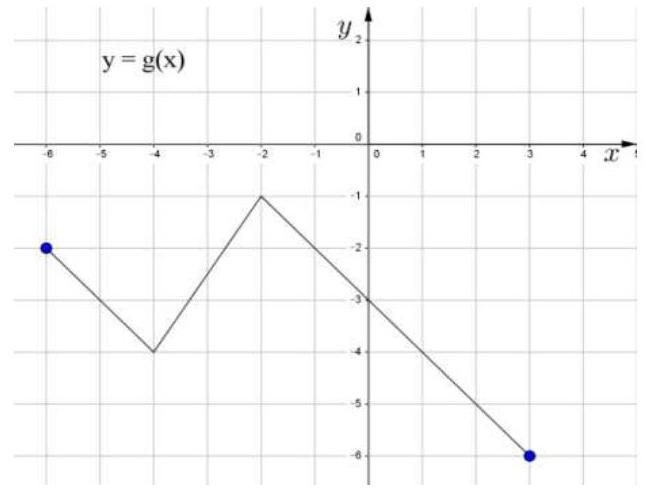
\includegraphics[max width=\textwidth, center]{2024_11_21_94f02db55673a8a7b820g-10(1)}

Wykres funkcji \(f\) przekształcono i otrzymano wykres funkcji \(g\), zatem:\\
A. \(g(x)=f(x-2)+3\)\\
B. \(g(x)=f(x+2)+3\)\\
C. \(g(x)=f(x-2)-3\)\\
D. \(g(x)=f(x+2)-3\)

\section*{Zadanie 22.}
Rozwiązaniem równania \(\frac{-2 x+6}{x-3}=x\) jest:\\
A. \(x_{1}=-2\)\\
B. \(x_{1}=-2, x_{2}=3\)\\
C. \(x_{1}=-3, x_{2}=2\)\\
D. \(x_{1}=3\)

\section*{Zadanie 23.}
Najmniejsza wartość funkcji kwadratowej \(f(x)=x^{2}-4 x-5\) w przedziale \(\langle-3,-1\rangle\) jest równa:\\
A. 4\\
B. -2\\
C. -9\\
D. 0

\section*{BRUDNOPIS}
\begin{center}

\includegraphics[max width=\textwidth]{2024_11_21_94f02db55673a8a7b820g-11}
\end{center}

\section*{ZADANIA OTWARTE}
Rozwiąania zadań o numerach od 24. do 34. nalė̇y zapisać w wyznaczonych miejscach pod treścia zadania.

\section*{Zadanie 24. (0-2)}
W trójkącie równobocznym \(A B C\) punkt \(D\) dzieli bok \(A C\) w stosunku \(|A D|:|D C|=2: 3\).\\
Oblicz tangens kąta \(A B D\).\\

\includegraphics[max width=\textwidth, center]{2024_11_21_94f02db55673a8a7b820g-12(11)}

\section*{Zadanie 25. (0-2)}
Rozwiąż nierówność \((x-2)(x-4) \geq 4(x+4)+3\).

\begin{center}
\begin{tabular}{|c|c|c|c|c|c|c|c|c|c|c|c|c|c|c|c|c|c|c|c|c|c|c|c|c|c|c|c|c|c|}
\hline
 &  &  &  &  &  &  &  &  &  &  &  &  &  &  &  &  &  &  &  &  &  &  &  &  &  &  &  &  &  \\
\hline
 &  &  &  &  &  &  &  &  &  &  &  &  &  &  &  &  &  &  &  &  &  &  &  &  &  &  &  &  &  \\
\hline
 &  &  &  &  &  &  &  &  &  &  &  &  &  &  &  &  &  &  &  &  &  &  &  &  &  &  &  &  &  \\
\hline
 &  &  &  &  &  &  &  &  &  &  &  &  &  &  &  &  &  &  &  &  &  &  &  &  &  &  &  &  &  \\
\hline
 &  &  &  &  &  &  &  &  &  &  &  &  &  &  &  &  &  &  &  &  &  &  &  &  &  &  &  &  &  \\
\hline
 &  &  &  &  &  &  &  &  &  &  &  &  &  &  &  &  &  &  &  &  &  &  &  &  &  &  &  &  &  \\
\hline
 &  &  &  &  &  &  &  &  &  &  &  &  &  &  &  &  &  &  &  &  &  &  &  &  &  &  &  &  &  \\
\hline
 &  &  &  &  &  &  &  &  &  &  &  &  &  &  &  &  &  &  &  &  &  &  &  &  &  &  &  &  &  \\
\hline
 &  &  &  &  &  &  &  &  &  &  &  &  &  &  &  &  &  &  &  &  &  &  &  &  &  &  &  &  &  \\
\hline
 &  &  &  &  &  &  &  &  &  &  &  &  &  &  &  &  &  &  &  &  &  &  &  &  &  &  &  &  &  \\
\hline
 &  &  &  &  &  &  &  &  &  &  &  &  &  &  &  &  &  &  &  &  &  &  &  &  &  &  &  & 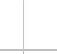
\includegraphics[max width=\textwidth]{2024_11_21_94f02db55673a8a7b820g-12(9)}
 &  \\
\hline
 &  &  &  &  &  &  &  &  &  &  &  &  &  &  &  &  &  &  &  &  &  &  &  &  &  &  &  &  &  \\
\hline
 &  &  &  &  &  &  &  &  &  &  &  &  &  &  &  &  &  &  &  &  &  &  &  &  &  &  &  &  &  \\
\hline
 &  &  &  &  &  &  &  &  &  &  &  &  &  &  &  &  &  &  &  &  &  &  &  &  & 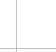
\includegraphics[max width=\textwidth]{2024_11_21_94f02db55673a8a7b820g-12(2)}
 &  &  & 
\includegraphics[max width=\textwidth]{2024_11_21_94f02db55673a8a7b820g-12(8)}
 &  \\
\hline
 &  &  &  &  &  &  &  &  &  &  &  &  &  &  &  &  &  &  &  &  &  &  &  &  & 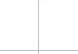
\includegraphics[max width=\textwidth]{2024_11_21_94f02db55673a8a7b820g-12(5)}
 &  &  & 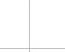
\includegraphics[max width=\textwidth]{2024_11_21_94f02db55673a8a7b820g-12(10)}
 &  \\
\hline
 &  &  &  &  &  &  &  &  &  &  &  &  &  &  &  &  &  &  &  &  &  &  &  &  &  &  &  &  &  \\
\hline
 &  &  &  &  &  &  &  &  &  &  &  &  &  &  &  &  &  &  &  &  &  &  &  &  & 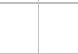
\includegraphics[max width=\textwidth]{2024_11_21_94f02db55673a8a7b820g-12(4)}
 &  &  & 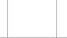
\includegraphics[max width=\textwidth]{2024_11_21_94f02db55673a8a7b820g-12}
 &  \\
\hline
 &  &  &  &  &  &  &  &  &  &  &  &  &  &  &  &  &  &  &  &  &  &  &  &  & 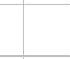
\includegraphics[max width=\textwidth]{2024_11_21_94f02db55673a8a7b820g-12(1)}
 &  &  & 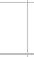
\includegraphics[max width=\textwidth]{2024_11_21_94f02db55673a8a7b820g-12(3)}
 &  \\
\hline
 &  &  &  &  &  &  &  &  &  &  &  &  &  &  &  &  &  &  &  &  &  &  &  &  & 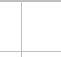
\includegraphics[max width=\textwidth]{2024_11_21_94f02db55673a8a7b820g-12(7)}
 &  &  &  &  \\
\hline
 &  &  &  &  &  &  &  &  &  &  &  &  &  &  &  &  &  &  &  &  &  &  &  &  &  &  &  & 
\includegraphics[max width=\textwidth]{2024_11_21_94f02db55673a8a7b820g-12(6)}
 &  \\
\hline
\end{tabular}
\end{center}

\section*{Zadanie 26. (0-2)}
Dane są trzy okręgi \(o_{1}, o_{2} i o_{3}\). Okręgi \(o_{1}, o_{2}\) są styczne zewnętrznie, jednocześnie są styczne wewnętrznie do okręgu \(o_{3}\) (patrz rysunek). Promienie okręgów \(o_{1} i \quad o_{2}\) są odpowiednio równe \(r_{1}\) i \(r_{2}\), a środki wszystkich trzech okręgów leżą na jednej prostej. Uzasadnij, że długość odcinka \(E F\) jest równa \(4 \sqrt{r_{1} r_{2}}\), gdzie odcinek \(E F\) jest cięciwą okręgu \(o_{3}\) i zawiera się w wspólnej stycznej okręgów \(o_{1} i \quad o_{2}\).\\
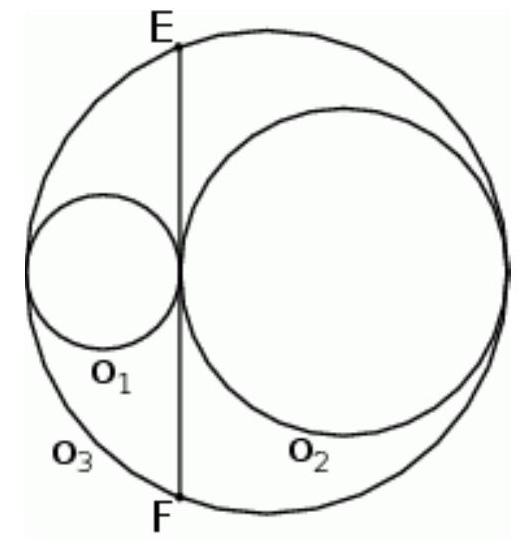
\includegraphics[max width=\textwidth, center]{2024_11_21_94f02db55673a8a7b820g-13}\\

\includegraphics[max width=\textwidth, center]{2024_11_21_94f02db55673a8a7b820g-13(1)}

\section*{Zadanie 27. (0-2)}
Różnica ciągu arytmetycznego jest równa ( -3 ), a szósty wyraz jest równy 3012. Oblicz \(S_{2017}\).\\

\includegraphics[max width=\textwidth, center]{2024_11_21_94f02db55673a8a7b820g-14}

\section*{Zadanie 28. (0-2)}
Uzasadnij, że suma trzech kolejnych potęg liczby 2 o wykładnikach całkowitych dodatnich jest podzielna przez 14.

\begin{center}
\begin{tabular}{|c|c|c|c|c|c|c|c|c|c|c|c|c|c|c|c|c|c|c|c|c|c|c|c|c|c|c|c|c|c|c|c|}
\hline
 &  &  &  &  &  &  &  &  &  &  &  &  &  &  &  &  &  &  &  &  &  &  &  &  &  &  &  &  &  &  &  \\
\hline
 &  &  &  &  &  &  &  &  &  &  &  &  &  &  &  &  &  &  &  &  &  &  &  &  &  &  &  &  &  &  &  \\
\hline
 &  &  &  &  &  &  &  &  &  &  &  &  &  &  &  &  &  &  &  &  &  &  &  &  &  &  &  &  &  &  &  \\
\hline
 &  &  &  &  &  &  &  &  &  &  &  &  &  &  &  &  &  &  &  &  &  &  &  &  &  &  &  &  &  &  &  \\
\hline
 &  &  &  &  &  &  &  &  &  &  &  &  &  &  &  &  &  &  &  &  &  &  &  &  &  &  &  &  &  &  &  \\
\hline
 &  &  &  &  &  &  &  &  &  &  &  &  &  &  &  &  &  &  &  &  &  &  &  &  &  &  &  &  &  &  &  \\
\hline
 &  &  &  &  &  &  &  &  &  &  &  &  &  &  &  &  &  &  &  &  &  &  &  &  &  &  &  &  &  &  &  \\
\hline
 &  &  &  &  &  &  &  &  &  &  &  &  &  &  &  &  &  &  &  &  &  &  &  &  &  &  &  &  &  &  &  \\
\hline
 &  &  &  &  &  &  &  &  &  &  &  &  &  &  &  &  &  &  &  &  &  &  &  &  &  &  &  &  &  &  &  \\
\hline
 &  &  &  &  &  &  &  &  &  &  &  &  &  &  &  &  &  &  &  &  &  &  &  &  &  &  &  &  &  &  &  \\
\hline
 &  &  &  &  &  &  &  &  &  &  &  &  &  &  &  &  &  &  &  &  &  &  &  &  &  &  &  &  &  &  &  \\
\hline
 &  &  &  &  &  &  &  &  &  &  &  &  &  &  &  &  &  &  &  &  &  &  &  &  &  &  &  &  &  &  &  \\
\hline
 &  &  &  &  &  &  &  &  &  &  &  &  &  &  &  &  &  &  &  &  &  &  &  &  &  &  &  &  &  &  &  \\
\hline
 &  &  &  &  &  &  &  &  &  &  &  &  &  &  &  &  &  &  &  &  &  &  &  &  &  &  &  &  &  &  &  \\
\hline
 &  &  &  &  &  &  &  &  &  &  &  &  &  &  &  &  &  &  &  &  &  &  &  &  &  &  &  &  &  &  &  \\
\hline
 &  &  &  &  &  &  &  &  &  &  &  &  &  &  &  &  &  &  &  &  &  &  &  &  &  &  &  &  &  &  &  \\
\hline
 &  &  &  &  &  &  &  &  &  &  &  &  &  &  &  &  &  &  &  &  &  &  &  &  &  &  &  &  &  &  &  \\
\hline
 &  &  &  &  &  &  &  &  &  &  &  &  &  &  &  &  &  &  &  &  &  &  &  &  &  &  &  &  &  &  &  \\
\hline
\end{tabular}
\end{center}

\section*{Zadanie 29. (0-2)}
Przekątna \(A C\) czworokąta \(A B C D\) zawiera się w prostej o równaniu \(x-2 y-7=0\).\\
Wierzchołki \(B, D\) tego czworokąta mają współrzędne \(B=(8 ;-6), D=(-3 ; 5)\). Oblicz współrzędne punktu przecięcia się przekątnych czworokąta \(A B C D\).\\

\includegraphics[max width=\textwidth, center]{2024_11_21_94f02db55673a8a7b820g-15}

\section*{Zadanie 30. (0-2)}
Ze zbioru liczb \(\{1,2,3,4,5,6,7,8,9,10\}\) losujemy bez zwracania kolejno dwie liczby i od pierwszej odejmujemy drugą. Oblicz prawdopodobieństwo zdarzenia, że otrzymana w ten sposób różnica liczb jest większa od 2.\\

\includegraphics[max width=\textwidth, center]{2024_11_21_94f02db55673a8a7b820g-16}

\section*{Zadanie 31. (0-4)}
Oblicz pole i obwód trapezu prostokątnego, w którym podstawy mają długości 13 cm i 22 cm , a tangens kąta ostrego jest równy \(1 \frac{1}{3}\).\\

\includegraphics[max width=\textwidth, center]{2024_11_21_94f02db55673a8a7b820g-17}

\section*{Próbny egzamin maturalny z matematyki}
\section*{Zadanie 32. (0-5)}
W ciągu geometrycznym \(\left(a_{n}\right)\) dane są iloraz \(q=-\frac{1}{2}\) oraz suma \(a_{12}+a_{13}+\cdots+a_{24}=\frac{7 \cdot\left(2^{13}+1\right)}{3 \cdot 2^{23}}\). Oblicz \(x\), dla którego ciąg \(\left(a_{4}, x-a_{6}, a_{8}\right)\) jest ciągiem arytmetycznym.\\

\includegraphics[max width=\textwidth, center]{2024_11_21_94f02db55673a8a7b820g-18}

\section*{Zadanie 33. (0-4)}
Suma długości wszystkich krawędzi ostrosłupa prawidłowego trójkątnego jest równa 96, a krawędź boczna tworzy z płaszczyzną podstawy kąt, którego cosinus jest równy \(\frac{\sqrt{3}}{9}\). Oblicz pole powierzchni bocznej tego ostrosłupa.\\

\includegraphics[max width=\textwidth, center]{2024_11_21_94f02db55673a8a7b820g-19}

\section*{PESEL}
\begin{center}
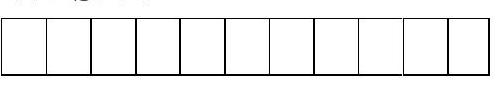
\includegraphics[max width=\textwidth]{2024_11_21_94f02db55673a8a7b820g-20(1)}
\end{center}

WYPELNIA ZDAJĄCY

\begin{center}
\begin{tabular}{|c|c|c|c|c|}
\hline
\multirow{2}{*}{\begin{tabular}{l}
Nr \\
zad. \\
\end{tabular}} & \multicolumn{4}{|c|}{Odpowiedzi} \\
\hline
 & A & B & C & D \\
\hline
1 & ㅁ & - & - & ㅁ \\
\hline
2 & ㅁ & - & ㅁ & ㅁ \\
\hline
3 & ㅁ & ㅁ & - & ㅁ \\
\hline
4 & ㅁ & ㅁ & ㅁ & ㅁ \\
\hline
5 & ㅁ & ㅁ & ㅁ & ㅁ \\
\hline
6 & ㅁ & ㅁ & ㅁ & ㅁ \\
\hline
7 & ㅁ & ㅁ & ㅁ & ㅁ \\
\hline
8 & ㅁ & ㅁ & ㅁ & ㅁ \\
\hline
9 & ㅁ & ㅁ & - & ㅁ \\
\hline
10 & ㅁ & ㅁ & ㅁ & - \\
\hline
11 & ㅁ & ㅁ & ㅁ & - \\
\hline
12 & ㅁ & ㅁ & ㅁ & - \\
\hline
13 & ㅁ & ㅁ & ㅁ & ㅁ \\
\hline
14 & ㅁ & ㅁ & - & ㅁ \\
\hline
15 & ㅁ & ㅁ & - & ㅁ \\
\hline
16 & ㅁ & ㅁ & ㅁ & ㅁ \\
\hline
17 & ㅁ & ㅁ & ㅁ & ㅁ \\
\hline
18 & ㅁ & ㅁ & ㅁ & ㅁ \\
\hline
19 & ㅁ & ㅁ & - & ㅁ \\
\hline
20 & ㅁ & ㅁ & - & ㅁ \\
\hline
21 & ㅁ & ㅁ & - & ㅁ \\
\hline
22 & ㅁ & ㅁ & - & - \\
\hline
23 & ㅁ & ㅁ & ㅁ & ㅁ \\
\hline
\end{tabular}
\end{center}

WYPELNIA EGZAMINATOR

\begin{center}
\begin{tabular}{|c|c|c|c|c|c|c|}
\hline
\multirow{2}{*}{\begin{tabular}{c}
Nr \\
zad. \\
\end{tabular}} & \multicolumn{6}{|c|}{Punkty} \\
\hline
 & \(\mathbf{0}\) & \(\mathbf{1}\) & \(\mathbf{2}\) & \(\mathbf{3}\) & \(\mathbf{4}\) & \(\mathbf{5}\) \\
\hline
\(\mathbf{2 4}\) & \(\square\) & \(\square\) & \(\square\) &  &  &  \\
\hline
\(\mathbf{2 5}\) & \(\square\) & \(\square\) & \(\square\) &  &  &  \\
\hline
\(\mathbf{2 6}\) & \(\square\) & \(\square\) & \(\square\) &  &  &  \\
\hline
\(\mathbf{2 7}\) & \(\square\) & \(\square\) & \(\square\) &  &  &  \\
\hline
\(\mathbf{2 8}\) & \(\square\) & \(\square\) & \(\square\) &  &  &  \\
\hline
\(\mathbf{2 9}\) & \(\square\) & \(\square\) & \(\square\) &  &  &  \\
\hline
\(\mathbf{3 0}\) & \(\square\) & \(\square\) & \(\square\) &  &  &  \\
\hline
\(\mathbf{3 1}\) & \(\square\) & \(\square\) & \(\square\) & \(\square\) & \(\square\) &  \\
\hline
\(\mathbf{3 2}\) & \(\square\) & \(\square\) & \(\square\) & \(\square\) & \(\square\) & \(\square\) \\
\hline
\(\mathbf{3 3}\) & \(\square\) & \(\square\) & \(\square\) & \(\square\) & \(\square\) &  \\
\hline
\end{tabular}
\end{center}

SUMA PUNKTÓW\\

\includegraphics[max width=\textwidth, center]{2024_11_21_94f02db55673a8a7b820g-20}


\end{document}